%%
%% This is file `sample-sigconf.tex',
%% generated with the docstrip utility.
%%
%% The original source files were:
%%
%% samples.dtx  (with options: `sigconf')
%% 
%% IMPORTANT NOTICE:
%% 
%% For the copyright see the source file.
%% 
%% Any modified versions of this file must be renamed
%% with new filenames distinct from sample-sigconf.tex.
%% 
%% For distribution of the original source see the terms
%% for copying and modification in the file samples.dtx.
%% 
%% This generated file may be distributed as long as the
%% original source files, as listed above, are part of the
%% same distribution. (The sources need not necessarily be
%% in the same archive or directory.)
%%
%%
%% Commands for TeXCount
%TC:macro \cite [option:text,text]
%TC:macro \citep [option:text,text]
%TC:macro \citet [option:text,text]
%TC:envir table 0 1
%TC:envir table* 0 1
%TC:envir tabular [ignore] word
%TC:envir displaymath 0 word
%TC:envir math 0 word
%TC:envir comment 0 0
%%
%%
%% The first command in your LaTeX source must be the \documentclass command.
\PassOptionsToPackage{svgnames}{xcolor}
\documentclass[dvipsnames,format=sigconf,anonymous=false,review=false]{acmart}
%%
%% \BibTeX command to typeset BibTeX logo in the docs
\AtBeginDocument{%
  \providecommand\BibTeX{{%
    \normalfont B\kern-0.5em{\scshape i\kern-0.25em b}\kern-0.8em\TeX}}}


%% These commands are for a PROCEEDINGS abstract or paper.
\copyrightyear{2024}
\acmYear{2024}
\setcopyright{rightsretained}
\acmConference[GECCO '24 Companion]{Genetic and Evolutionary Computation
Conference}{July 14--18, 2024}{Melbourne, VIC, Australia}
\acmBooktitle{Genetic and Evolutionary Computation Conference (GECCO '24
Companion), July 14--18, 2024, Melbourne, VIC, Australia}
\acmDOI{10.1145/3638530.3654415}
\acmISBN{979-8-4007-0495-6/24/07}

%%
%% end of the preamble, start of the body of the document source.
\begin{document}

%%
%% The "title" command has an optional parameter,
%% allowing the author to define a "short title" to be used in page headers.
\title[Generational Information Transfer with Neuroevolution on Control Tasks]{Generational Information Transfer \\with Neuroevolution on Control Tasks}

%%
%% The "author" command and its associated commands are used to define
%% the authors and their affiliations.
%% Of note is the shared affiliation of the first two authors, and the
%% "authornote" and "authornotemark" commands
%% used to denote shared contribution to the research.
\author{Maximilien Le Clei}
\affiliation{%
  \institution{Université de Montréal}
  \city{Montréal}
  \country{Canada}
}
\email{maximilien.le.clei@umontreal.ca}

\author{Stav Bar-Sheshet}
\affiliation{%
  \institution{Tel-Aviv University}
  \city{Tel Aviv}
  \country{Israel}
}
\email{stavb1@mail.tau.ac.il}

\author{Pierre Bellec}
\affiliation{%
  \institution{Université de Montréal}
  \city{Montréal}
  \country{Canada}
}
\email{pierre.bellec@umontreal.ca}

%%
%% By default, the full list of authors will be used in the page
%% headers. Often, this list is too long, and will overlap
%% other information printed in the page headers. This command allows
%% the author to define a more concise list
%% of authors' names for this purpose.
\renewcommand{\shortauthors}{Le Clei, et al.}

%%
%% The abstract is a short summary of the work to be presented in the
%% article.



\begin{abstract}
Traditional genetic algorithms compute fitness scores every generation for all agents in a population, which typically requires agents to perform a task until they either fail or succeed. These evaluations can turn into a computational bottleneck when tasks are either time-consuming or infinite. A common workaround is to set an expiration time on agent trials, i.e. to evaluate agents on a subset of the task, which can bias the true task objective. We propose to address this bias through a novel information inheritance genetic algorithm where three distinct attributes can be passed down generations: the task environment state (agents resume from where their parents reached task expiration), the memory state (agents inherit internal representations from their parents); and the fitness (ancestors evaluation scores are compounded with an agent's own score for selection). We benchmark the various combinations of these three inherited attributes by running a genetic neuroevolution algorithm on popular feature-based control tasks. We report that information inheritance can lead to substantial increases in both data and runtime efficiency, suggesting it may greatly benefit a variety of genetic algorithm techniques and applications in the future. We provide \textcolor{blue}{\href{https://github.com/courtois-neuromod/cneuromax/tree/gen_transfer}{the relevant source code}}.
\end{abstract}

\maketitle

\section{Background}
A standard genetic algorithm can be described as being composed of three stages: variation, evaluation and selection. In many genetic algorithms, the evaluation stage consumes most of the runtime. Indeed, while time-consuming variation and selection stages that significantly improve algorithm performance are hard to elaborate, granting additional runtime to the evaluation stage can reduce bias with respect to the true expected agent fitness scores \cite{lambora2019genetic, stanley2019designing}. Withholding time constraints, the optimal way to evaluate an agent on a given task is to have it perform the task until it either fails or succeeds. Additionally, if the evaluation protocol is stochastic, an agent needs to re-perform the task infinitely if we wish to obtain its true expected fitness. In real world scenarios, practitioners need to set an upper bound on the number of task roll-outs and the length of each roll-out. A common setup is therefore to evaluate on a single roll-out and set a reasonable expiration time \cite{salimans2017evolution, such2017deep} so that agents are exposed to most of the task content. However, this operation introduces a bias with the true task objective, resulting from task roll-outs repeatedly reaching time expiration. A trade-off therefore ensues between a lower bias and a shorter runtime.

\section{Introduction}

In this work, we introduce a framework to sidestep the aforedescribed runtime-bias trade-off by introducing an alternative way to evaluate agents. The main idea we propose is to not reset the task environment state after agents reach time expiration. Instead, we propose to have new generations of agents begin their evaluation protocol by resuming from their parent's final environment state. In order to help agents make sense of the environment state in which they find themselves, we propose to also transfer final memory states, that is, the internal representation(s) that an agent updates based on past experiences. Finally, when transferring the environment, agents no longer necessarily get evaluated on the same sections of a task as the other agents in their respective generation. We therefore propose to also transfer fitness information across generations, so that an agent’s fitness score becomes a combination of their own evaluation score plus that of their ancestors.

Optimizing the runtime efficiency of evolutionary algorithms is a hot topic \cite{evotorch2023arxiv, chalumeau2023qdax, evojax2022}, however the information inheritance literature is relatively sparse. While fitness inheritance has been studied in the past \cite{smith1995fitness}, to the best of our knowledge, environment and memory state transfer have not. In order to evaluate the proposed framework's performance, we performed experiments on the various ways in which the three transfer attributes (environment state, memory state \& fitness) can be combined. To do so, we 1) selected several tasks from the Gymnasium library \cite{towers_gymnasium_2023},  2) ran simple crossover-free genetic algorithms and 3) equipped agents with fixed-architecture recurrent neural networks. We report vastly increased data and runtime efficiency with minimal and easily correctable loss in performance.

\section{Generational Information Transfer} \label{methods}

\textbf{Transfer attributes.} In traditional genetic algorithms, only the genotype is transmitted from a parent to its children. We introduce three attributes of potential additional value if transferred between generations of agents:

\begin{itemize}

\item \textbf{The final environment state.} This transfer regime requires a time expiration hyper-parameter to represent the number of actions an agent produces before handing off the environment state to its children, if it is selected. We use the symbol \textbf{E} to represent this number of actions per evaluation and describe its three possible modes:

\begin{itemize}

\item \textbf{E=1}: Agents only perform one action during their evaluation. If selected, they transfer the environment state over to their children. This process goes on until an agent reaches task termination (success or failure). If that agent is selected, its children then begin their evaluation from a new, non-inherited environment state. 

\item \textbf{E=roll-out length}: All agents eventually reach task termination. Selected agents’ children start from a new, non-inherited environment state. Since no environment state is ever transferred, this is a regular genetic algorithm.

\item \textbf{E=k}: The behaviour is similar to \textbf{E=1}, however, agents can reach task termination before performing their \textbf{k} actions. In that case, we propose to reset the environment state, perform the remaining number of actions and save the resulting environment state. 

\end{itemize}

\item \textbf{The final memory state.} This is the final information held by an agent in memory upon evaluation termination (e.g., the final hidden state of a recurrent network). A more complicated operation could be to select and/or process from that memory state, however for simplicity we propose to transfer it as is. This transfer mode is mostly meant to be used in conjunction with the environment state transfer operation in order to transfer memory states within task roll-outs.

\item \textbf{The fitness.} By transferring agent fitness scores, we mean taking the evaluation scores of an agent's predecessors into account when calculating its own fitness. We propose a straightforward inheritance operation that simply adds all evaluation scores obtained by an agent's predecessors to its own evaluation score.

\end{itemize}

\textbf{Transfer modes.} We now introduce all the different ways that transfer attributes can be combined and we discuss some potential drawbacks and benefits of these information transfer attributes on agent performance and selection.

\begin{enumerate}

\item \textbf{Environment state only (\textcolor{red}{env} \normalfont in Figure \ref{output.png}\textbf{).}} We anticipate three potentially negative consequences of transferring the environment state by itself:
\begin{enumerate}
\item Unless a task is fully observable, agents are systematically introduced to environment states that came about through interactions with the agents’ ancestors. With a freshly initialized memory state, the newer agents cannot recall those interactions and have to rely on their own experience in order to make sense of their situation.
\item If the task length is variable, agents can end up in task sections that produce relatively lower reward signals than other agents in their generation. As such, agents can receive lower, potentially eliminatory fitness scores, irrespective of their true expected fitness.
\item Since transferring the environment state typically involves evaluating and selecting agents based on smaller task portions than a traditional genetic algorithm, greedy agent behaviour is more readily rewarded with respect to the immediate next selection operation. 
\end{enumerate}

As a result of the above-mentioned properties, a task state-only transfer mode appears to be theoretically bounded in performance by standard genetic algorithms. However, if performance on the different task sections is reflective of overall task performance, the fact that we can now run more generations given the same compute budget could increase data/runtime efficiency up to the theoretical bound.

\item \textbf{Fitness only (\textcolor{Green}{fit}).} Increased performance or data/runtime efficiency with this transfer mode implies that the leeway obtained by higher scoring lineages to explore harmful short-term mutations has evolutionary value for the task at hand.

\item \textbf{Memory state only (\textcolor{Blue}{mem}).} This transfer mode was originally introduced as a complement to transferring the environment state and meant to be performed \textbf{within} a single task roll-out. When environment state transfer does not occur, meaning that agents perform full roll-outs, we propose an alternative operation that transfers memory states \textbf{across} task roll-outs (without environment state transfer). Improved data efficiency/performance could indicate that the memory state is being successfully utilized to encode useful logic that builds on top of the existing network parameter-based logic.

\item \textbf{Environment state and fitness (\textcolor{DarkRed}{env+fit}).} One property of transferring the environment state is that, within a single generation, different agents can be evaluated on separate task sections. As mentioned in drawback (b) of the \textcolor{red}{env} transfer mode, this feature causes issues when different task sections yield different reward returns. Transferring fitness scores across generations should mitigate this issue by accounting for performance on the previous task sections, experienced by the agent’s ancestors.
 
\item \textbf{Environment state and memory state (\textcolor{Indigo}{env+mem}).} Another property of transferring the environment state is that new agents often no longer start a task from scratch. As mentioned in drawback (a) of the \textcolor{red}{env} transfer mode, this feature can be problematic if environments aren't fully observable. Indeed, in such cases, agents can be introduced to intermediate environment states with no information on how these states came about. Transferring memory states across generations gives agents a chance to mitigate this issue by encoding and transferring past experiences.

\item \textbf{Fitness and memory state (\textcolor{DarkCyan}{fit+mem}).} As the two transfer attributes seem orthogonal in functionality, the combination result should be some function of two independent factors.

\item \textbf{Environment state, fitness and memory state\\(\textcolor{Goldenrod}{env+fit+mem}).} This information transfer mode comprises all three information attributes. It mitigates both the performance evaluation and resumability drawbacks (a \& b) of the \textcolor{red}{env} transfer mode by combining the solutions of the \textcolor{DarkRed}{env+fit} and \textcolor{Indigo}{env+mem} transfer modes.
\end{enumerate}

\textbf{Remarks on transferring the environment state.} We remark that not all reward functions work well with the environment state transfer operation. First, as a consequence of drawback (c) of the \textcolor{red}{env} transfer mode, exploration is more strongly discouraged than in a traditional genetic algorithm. Secondly, certain unexpected behaviours can result from applying this framework. Let us imagine a task for which the expected value of reward signals is higher during the early stages of a task roll-out. When possible, a sensible solution for an agent could be to purposely cause termination, if the penalty of doing so is overshadowed by the later rewards it will accumulate. Finally, certain reward functions are by default incompatible with the framework. For example, in the task CartPole-v1 from the Gymnasium library \cite{towers_gymnasium_2023}, agents are tasked with balancing a pole and are rewarded +1 for every time-step of the task roll-out. The task either terminates due to the pole having become unbalanced (failure) or due to reaching 500 time-steps of the pole staying balanced (success), with a reward of +1 still being granted in both cases. For \textbf{E=k}, agents forever have a fitness of \textbf{k}. Natively, such reward function is thus incompatible with the environment transfer operation (see the Discussion section for possible remedies).

\begin{figure*}
\vspace{-1em}
\centering
\centerline{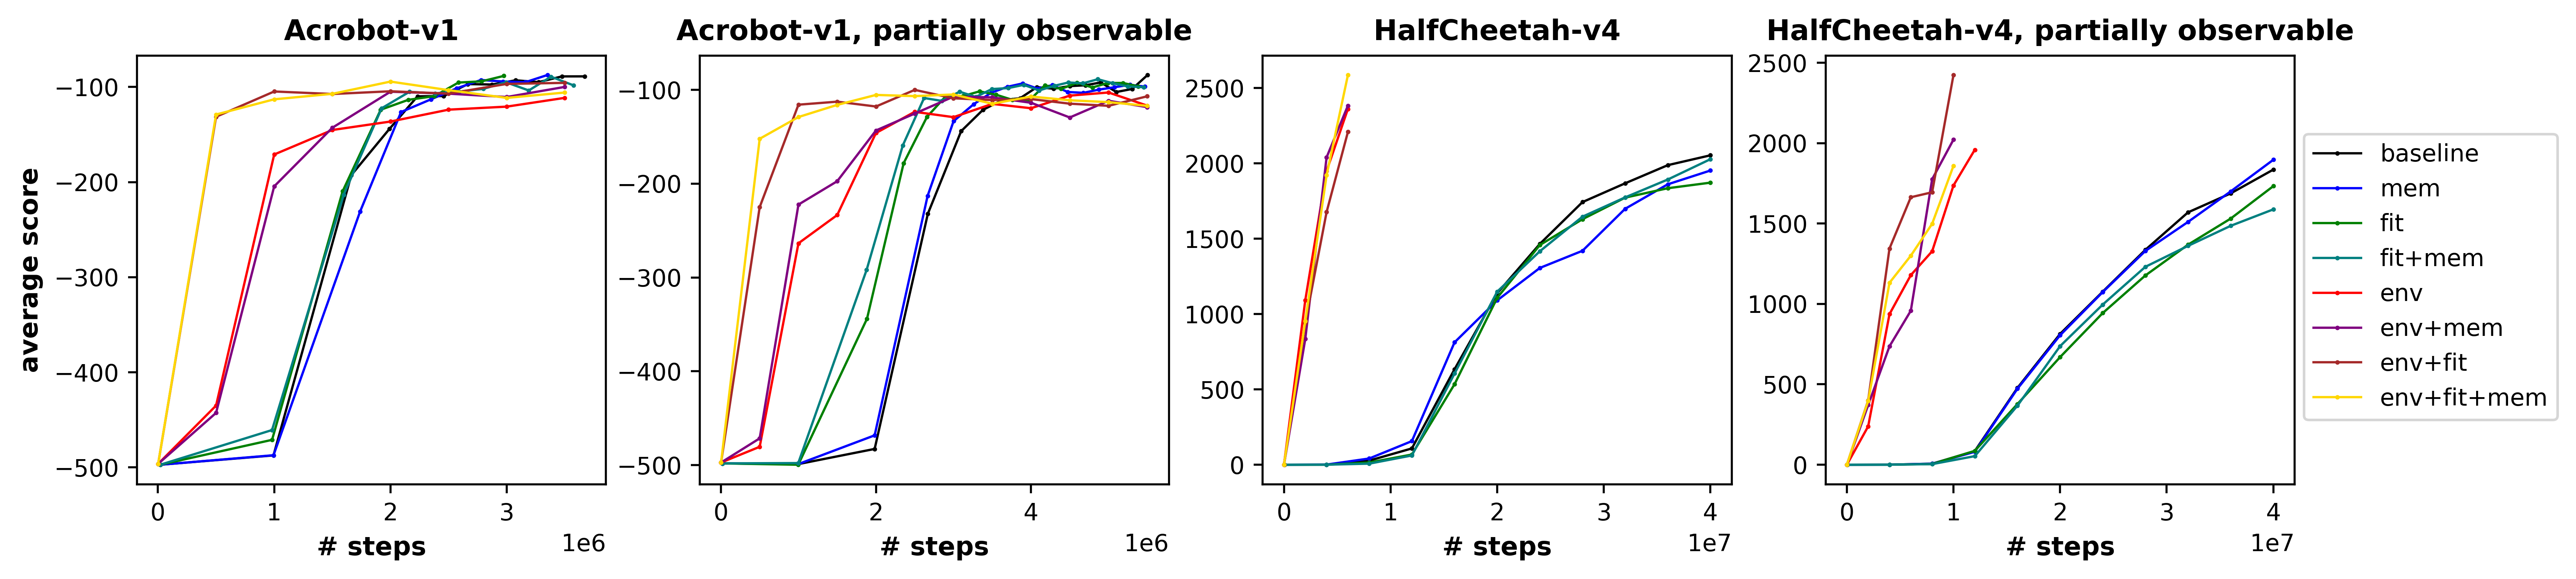
\includegraphics[width=\textwidth]{output.png}}
\vspace{-1em}
\caption{Average score over total number of state changes. \normalfont Progression of the mean population scores, averaged over 3 task instances never observed during optimization. Across all tasks, transferring the environment state yields increased data efficiency up to a ceiling of performance. Transfering the fitness always improves the environment state transfer operation. Transfering the memory state marginally improves the environment state transfer operation on partially observable tasks.}

\label{output.png}
\end{figure*}
\section{Experiments}

\textbf{Benchmarks.} We benchmarked all the combinations between the three generational transfer attributes. For that purpose, we ran experiments on two feature-input control tasks available in Gymnasium: Acrobot-v1 \& HalfCheetah-v4. In Acrobot-v1, agents receive position and velocity information from components of a double-link chain hanging from a fixed point. Agents must infer whether to apply a fixed positive, negative or null torque to the chain joint (discrete action). The reward function outputs a negative reward of -1 until the chain reaches a certain height, at which point the task terminates and a reward of 0 is given to indicate success. In HalfCheetah-v4, agents receive position and velocity information from various body components of a 2D robot resembling a cheetah. From this information, agents must infer different amounts of torque to apply to the various body rotors (continuous actions). The reward function output at every time-step is a sum of 1) a positive signal from the forward movement since the previous step and 2) a negative signal proportional to the amount of torque applied to the rotors, so as to encourage efficient energy use. As both tasks appear to be strongly observable (both position and velocity information are present in the inputs), memory information could be redundant. Therefore, we also benchmarked a version of each task for which the velocity information is hidden from the agent  \cite{morad2023popgym}.

\textbf{Algorithm.} We specified our neuroevolution algorithm with hyper parameters and design decisions commonly found in the literature \cite{salimans2017evolution, such2017deep, leclei2022neuroevolution}. We used a simple genetic algorithm with 50\% truncation selection over a population size of 40 agents. We equipped agents with neural networks of size \textit{(num\_inputs, 50, num\_outputs)} composed of one recurrent layer with tanh activations followed by one feed-forward layer. We perturbed all weights and biases by values drawn from $\mathcal{N}(0,0.01)$ during variation. During evaluation, we transformed input values by performing a running standardization. We also transformed network output values. For tasks with a discrete action space, we took the softmax of the network outputs and sampled the action according to the resulting probabilities. For tasks with a continuous action space, we applied tanh activations to the network outputs and then scaled the [-1,1] range to the [\textit{min\_action\_value, max\_action\_value}] range for each action. 

\textbf{Hyperparameter E.} Finally, we set the hyper-parameter \textbf{E} when transferring the environment state. Of note, setting the hyper-parameter \textbf{E} too low exacerbates drawback (c) introduced in the methods and further deviates the evaluation criterion from the true task objective. Setting the hyper-parameter \textbf{E} too high decreases the potential data/runtime efficiency gains from the environment transfer. We chose to set \textbf{E} to 1/10th of the maximum runtime for both tasks: 50 for Acrobot-v1 which terminates at 500 steps and 100 for HalfCheetah-v4 which terminates at 1000 steps.

\section{Results}

Throughout this section, we use the terms:

\begin{itemize}
\item “average score”:  refers to the mean score of the entire population (post-selection) over 3 task roll-outs seeded with integers never used during the optimization process.
\item “total number of steps”:  refers to the number of times an environment state has been changed as a result of an agent action, in gym terms: \texttt{env.step(action)}, summed over all agents that have ever been created and evaluated throughout the optimization process.
\end{itemize}

In Figure \ref{output.png} we plot the evolution of the average score over the total number of environment steps for all 4 tasks. More specifically, we first record the baseline’s (a standard genetic algorithm) highest average score after 1000 generations and plot its evolution towards that score. For each following transfer mode we then plot until one of the following two conditions is met: 1) the average score is higher than the maximum average score obtained by the baseline or 2) the total number of steps reaches the total number of steps realized by the baseline at its maximum average score.

We notice the following patterns in all experiments:
\begin{itemize}

\item Transferring the environment state always results in faster convergence. Our interpretation is that, for all tasks, the agent’s performance on task subsets is related to true task performance, which allows the algorithm to generate relevant representations. Separate analysis uncovered that the final median number of generations is between 1.5 to 4.5 times greater when transferring the environment state.

\item As expected, transferring the memory state is more valuable when the environment is partially rather than fully observable. In partially observable environments, memory transfer achieves performances marginally superior to not transferring the memory state, whenever transferring the environment state.

\item Transferring the fitness was always found to be beneficial whenever transferring the environment state.

\end{itemize}

Whenever the environment state is not transferred, we also note that the superiority of a transfer mode over the baseline is task-dependent: all such transfer modes are marginally superior for both Acrobot tasks, but inferior for the HalfCheetah tasks.

Furthermore, we notice the final performance gap, discussed in the methods, when the environment state is transferred for the Acrobot tasks. We however do not notice the performance gap for the HalfCheetah tasks. We believe that this is due to the HalfCheetah experiments not having converged despite running for one order of magnitude more steps than the Acrobot tasks. For the HalfCheetah tasks, the environment transfer modes reach the baseline maximum average score around 4x to 6x faster for the partially and strongly observable tasks, respectively. For the Acrobot tasks, the best state task transfer modes reach within percentages of the baseline maximum average score around 3x faster.

\section{Discussion}

We first wish to discuss the discrepancy between the gained data / runtime efficiency on the Acrobot tasks and on the HalfCheetah tasks, when transferring the environment state. We believe that one principal reason is the evolving length of Acrobot task roll-outs. While we set the hyper-parameter \textbf{E} to be constant across an experiment, Acrobot roll-outs become shorter as agents master the task, going from 500 time-steps with random agents to under 100 timesteps with optimal agents. As a result, the 1/10 time-steps to \textbf{E} ratio turns into a 1/2 ratio. In contrast, HalfCheetah roll-outs remain constant at 1000 time-steps, meaning the time-steps to \textbf{E} remains constant at 1/10.

Next, we wish to propose a solution to the performance gap with the maximum baseline average score when introducing the environment state transfer operations. We observed this gap on the Acrobot tasks and would have most likely observed it on HalfCheetah if all modes were run to convergence. First of all, we observe that the gap, as a percentage of a normalized score obtained by subtracting the score on generation \#1 to the maximum baseline average score is quite minimal. As a result, it seems quite probable that many of the representations acquired when transferring the environment state could be leveraged. We believe this hypothesis to be even more plausible when transferring the memory state in addition to the environment state as it better mirrors a standard task roll-out. Therefore, halting an experiment running the environment state transfer operation when hitting a plateau and fine-tuning the final population for several generations on a standard genetic algorithm seems like a reasonable decision. Some of the data/runtime efficiency would be erased, however it seems probable baseline-level performance could be achieved.

Finally, we wish to address the incompatibility of the environment state transfer with certain reward functions, which we first introduced in Section \ref{methods} when presenting the environment state transfer operation. We believe that many (but not all) reward functions can be modified so as to be compatible with the framework, without modifying optimal agent behaviour. We propose to carry on with the CartPole example introduced in Section \ref{methods}. One simple modification to the reward function that we believe would not alter optimal agent behaviour is simply to not grant the final positive reward signal if the task is failed. As such, agents that fail the task would obtain a maximal evaluation score of \textbf{k-1} and thus face selection pressure in the presence of agents that did not fail during their own evaluation. Ultimately, we notice that different task reward functions come with different out-of-the-box incompatibilities with the framework. As such, we advise careful examination of the reward function with respect to the framework for any task.
\\
\vspace{-1em}
\section{Conclusion}

We have introduced a genetic algorithm framework to speed up optimization by shortening agent evaluation and transferring relevant information across generations. We benchmarked this framework through neuroevolution on four popular control tasks. We observed significant improvements in data/runtime efficient convergence with minimal loss of performance across all tasks. Finally, we discussed a simple way to address the decrease in performance by sacrificing some of the gained efficiency. We believe that future work on time-consuming task optimization could greatly benefit from applying this framework. 







\renewcommand*{\bibfont}{\scriptsize}
\bibliographystyle{ACM-Reference-Format}
{\footnotesize
\bibliography{refs}}
\vspace{-3em}
\end{document}
\endinput
%%
%% End of file `sample-sigconf.tex'.
